\documentclass[11pt]{article}

\usepackage[margin=1in]{geometry}
\usepackage{amsmath,amssymb,amsfonts}
\usepackage{amsthm}
\usepackage{graphicx}
\usepackage{hyperref}
\usepackage{bm}
\usepackage{caption}
\usepackage{cite}
\usepackage{kotex}
\usepackage{listings}
\usepackage{xcolor}

\definecolor{codegreen}{rgb}{0,0.6,0}
\definecolor{codegray}{rgb}{0.5,0.5,0.5}
\definecolor{codepurple}{rgb}{0.58,0,0.82}
\definecolor{backcolour}{rgb}{0.95,0.95,0.92}

\lstdefinestyle{mystyle}{
    backgroundcolor=\color{backcolour},   
    commentstyle=\color{codegreen},
    keywordstyle=\color{magenta},
    numberstyle=\tiny\color{codegray},
    stringstyle=\color{codepurple},
    basicstyle=\ttfamily\footnotesize,
    breakatwhitespace=false,         
    breaklines=true,                 
    captionpos=b,                    
    keepspaces=true,                 
    numbers=left,                    
    numbersep=5pt,                  
    showspaces=false,                
    showstringspaces=false,
    showtabs=false,                  
    tabsize=2
}

\lstset{style=mystyle}

\title{사회적 스트레스 역학의 규모의 역설:\\
진화적 불일치, 정책 체제, 네트워크 이득, 그리고 마지노 시간}

\author{정선철\\[4pt]
\small \texttt{zotanika@gmail.com}
}
\date{\today}

\theoremstyle{plain}
\newtheorem{assumption}{가정}
\newtheorem{proposition}{명제}

\begin{document}
\maketitle

\begin{abstract}
본 연구는 정보 이론, 제어 이론, 그리고 정책 체제 모델을 융합하여, 사회적 스트레스 역학을 설명하는 새로운 이론적 틀을 제시한다.
우리는 인간의 공감을, \textbf{물리적 시공간에 뿌리를 둔 소규모 대면 공동체}에서 분산과 스트레스를 흡수하기 위해 진화한 \textbf{`국소적 감쇠 기제(local damping mechanism)'}로 이해한다.
그러나 지연 시간이 거의 없고 전역적인 도달 범위를 가진 현대의 초연결 네트워크---특히 디지털 환경---에서, 이 기제는 역설적으로 ``진화적 불일치(evolutionary mismatch)''를 야기할 수 있다.

이러한 불일치를 배경으로, 본 연구는 두 가지 이상적인 정책/문화적 대응 양상을 비교 분석한다:
(1) 개인의 자율성과 문제 해결을 장려하고, 적절한 스트레스를 학습과 역량 확장의 발판으로 삼는 \textbf{적응형/자율 중심 체제}(사회 A);
(2) 공감, 보호, 외부 지원을 강조하며, 시스템 수준에서 개인의 스트레스를 빠르게 완충하는 데 주력하는 \textbf{지원 중심 체제}(사회 B).
두 사회는 동일한 공감 분포와 동일한 초기 심리적 회복탄력성 분포를 공유한다.

우리는 \textbf{인지 스트레스}를 공감($E$), 네트워크 결합($G$), 그리고 정책 체제의 함수로 정의한다. 이 요인들이 상호작용하여 어떻게 회복탄력성과 \textbf{집단화(정체성 클러스터링)}의 역학을 형성하는지, 간단한 차분 방정식을 통해 모델링한다.
국소적 위상과 `좁은 세상(Small-World)' 효과를 반영한 에이전트 기반 시뮬레이션 결과, 동일한 초기 조건과 외부 자극 하에서도 사회 A와 사회 B는 시간이 지남에 따라 극명하게 다른 궤적을 보인다.
사회 A는 높은 회복탄력성 균형으로 수렴하는 반면, 사회 B는 평균 회복탄력성 하락과 집단화의 심화를 겪는 경향이 나타난다.

나아가 구체적인 이분법적 모델을 넘어, 스트레스가 공감/집단화의 단조 함수로 생성되고, 회복탄력성이 갱신되는 보다 추상적인 프레임워크를 구축한다.
우리는 약한 구조적 가정 하에서 일반적인 단조성 결과를 증명한다: 어떠한 정책 체제나 공감 분포 하에서도, 집단화 수준을 낮게 유지하는 궤적은 모든 시점에서 더 높은 회복탄력성과 늦은 붕괴 시점을 보장한다.
이 추상적 모델 내에서 평균 회복탄력성이 임계값 이하로 떨어지는 시점을 \textbf{``마지노 시간($t_{\text{mag}}$)''}이라 정의하며, 구조적으로 집단 해체를 장려하는 정책은 이 임계점 도달을 반드시 지연시킴을 보인다.

본 모델은 현실을 단순화한 것이며 특정 국가나 이데올로기를 묘사하지 않는다. 오히려 공감, 네트워크 이득, 집단화, 그리고 정책이 상호작용하여 어떻게 장기적인 사회적 취약성을 축적시키는지, 그 구조적 메커니즘을 조명하는 데 목적이 있다.
\end{abstract}

\section{서론}

현대 사회는 다양한 형태의 취약성에 직면해 있다. 극심한 양극화, 만성적 스트레스, 사소한 갈등의 폭발적 확대가 그 예다.
흔히 공론장과 학계는 이 문제를 도덕적 혹은 이데올로기적 렌즈로 틀 짓곤 한다:
누가 옳고 그른가?  
공감이 너무 적은가, 아니면 너무 많은가?  
특정 반응이 ``옳은가'' 아니면 ``그른가''?

사회과학의 실증적 연구는 설문과 빅데이터 분석을 통해 날로 정교해지고 있다.
그러나 서로 다른 정책 기조와 네트워크 구조 하에서 스트레스와 회복탄력성이 시간의 흐름에 따라 어떻게 \emph{공진화(co-evolve)} 하는지 설명하는 명시적인 \textbf{동역학(dynamic)} 모델은 여전히 드물다.

복잡계 이론과 진화생물학적 관점에서, 이 문제는 도덕성이 아닌 \textbf{구조와 역학}의 문제로 재해석될 수 있다.
우리는 이를 \textbf{`진화적 불일치(evolutionary mismatch)'}~\cite{lloyd2011evolutionary}의 특수한 사례로 본다.
공감을 포함한 인간의 심리 기제는 \textbf{물리적 시공간에 뿌리를 둔 소규모 대면 공동체}에서 형성되었다.
그 환경에서 공감은 개인의 스트레스를 집단으로 분산시켜 붕괴를 막는, 효과적인 `국소적 충격 흡수 장치'였다.

하지만 디지털 기술은 상호작용의 위상(topology)을 근본적으로 바꾸어 놓았다.
물리적 지연은 사라졌고 연결성은 폭발했다.
제어 이론 관점에서 이는 사회적 신호 처리의 \textbf{루프 이득(loop gain)}이 급증했음을 의미한다.
낮은 이득에서는 안정적이던 피드백 루프가, 높은 이득에서는 시스템 전체를 진동시키거나 발산시킬 수 있다는 것은 공학의 기본 원리다.

이러한 구조적 변동을 배경으로, 사회가 스트레스를 \emph{해석하고 관리}하는 방식은 크게 두 갈래로 나뉜다.
한쪽(사회 A)은 자율과 자기 조절을 강조하고, 다른 쪽(사회 B)은 보호와 공감, 외부 지원을 중시한다.
두 접근 모두 선한 의도를 담고 있지만, 고이득 네트워크 환경과 결합될 때 장기적 역학은 판이하게 달라질 수 있다.

본 연구는 Shannon의 채널 용량~\cite{shannon1948}, 시스템 다이내믹스~\cite{forrester1961,forrester1971}, Pentland의 사회 물리학~\cite{pentland2014}에서 영감을 얻어, 공감과 네트워크 이득, 정책이 어떻게 사회적 회복탄력성과 연결되는지 최소한의 동역학 모델로 구현한다.
우리는 먼저 구체적인 이분법적 모델을 분석하고, 이를 일반화하여 ``집단화를 억제하는 정책 경로가 체제의 세부 사항과 무관하게 회복탄력성을 개선하고 붕괴를 지연시킨다''는 단조성 결과를 증명한다.
우리의 목표는 단순한 데이터 피팅이 아니라, 초연결 사회의 구조적 취약성을 통찰할 수 있는 간결하고 형식적인 렌즈를 제공하는 것이다.

\section{정보 및 제어 이론적 관점}

\subsection{채널 용량과 사회적 대역폭}

Shannon~\cite{shannon1948}은 신호 전력 $S$, 노이즈 전력 $N$, 대역폭 $B$를 가진 통신 채널의 용량 $C$가 다음과 같음을 보여주었다:
\begin{equation}
C = B \log_2\left(1 + \frac{S}{N}\right).
\end{equation}

이를 사회적 맥락에 비유하면 다음과 같다:
\begin{itemize}
  \item $S$: 사회의 문제 해결 역량 및 제도적 처리 역량;
  \item $N$: 사회적 스트레스, 갈등, 그리고 감정적 노이즈;
  \item $B$: 공적 담론의 대역폭(미디어, 제도적 관심, 시민들의 인지적 대역폭).
\end{itemize}

중요한 점은 여기서의 ``노이즈'' $N$이 외생적인 백색 소음이 아니라는 점이다.
이는 시스템 내부에서 발생한다: 인지된 노이즈는 (1) 인구의 공감 분포와 (2) 네트워크 위상이 스트레스 신호를 어떻게 증폭하거나 감쇠시키느냐에 따라 달라진다.

\subsection{피드백 이득 요소로서의 공감}

본 연구에서 공감은 단순한 미덕을 넘어, 사회 시스템의 \textbf{피드백 이득 요소(feedback gain element)}로 재정의된다.
즉, 높은 공감이란 타인의 감정 상태와 스트레스 신호에 대한 민감도가 높음을 의미한다.

\begin{itemize}
  \item \textbf{약하게 결합된 네트워크 (국소적 감쇠).}  
  연결이 드물고 지연 시간이 긴 환경에서는, 개인의 스트레스가 소수 이웃과 공유된 후 소멸한다.
  이때 공감은 스트레스를 국소적으로 분산시키는 \textbf{음의 피드백(negative feedback)} 기제로 작용한다.

  \item \textbf{강하게 결합된 네트워크 (전역적 공명).}  
  연결이 조밀하고 즉각적인 환경에서는, 스트레스 신호가 광범위하게 급속 전파된다.
  고공감 개인들은 이 신호를 흡수하여 2차 스트레스를 겪고 이를 재송출한다.
  루프 이득이 일정 수준을 넘어서면, 공감은 스트레스를 증폭시키는 \textbf{양의 피드백(positive feedback)} 루프의 일부로 돌변한다.
\end{itemize}

이는 오디오 시스템의 라센 효과(Larsen effect, 하울링)와 유사하다: 마이크 자체가 ``나쁜'' 것은 아니지만, 이득과 피드백 경로가 특정 방식으로 구성되면 제어 불가능한 굉음(howling)을 발생시키는 데 기여하게 된다.

\section{수학적 모델: 두 정책 체제}
\label{sec:model}

이 절에서는 스트레스와 회복탄력성 역학을 설명하는 이분법적 모델을 구체화한다.
이어지는 4절에서는 이 모델을 포괄하는 추상적 프레임워크를 통해 일반적인 구조적 결론을 도출한다.

\subsection{인지 스트레스}
시간 $t$에서 개인 $i$의 \textbf{인지 스트레스} $S_i(t)$를 다음과 같이 정의한다:
\begin{equation}
S_i(t) = E_i^{\alpha} \bigl( 1 + \beta G_t \bigr),
\label{eq:stress}
\end{equation}
여기서
\begin{itemize}
  \item $E_i \sim P(E)$: 개인 $i$의 공감 수준(사회적 신호에 대한 민감도),
  \item $G_t \in [0,\infty)$: 시간 $t$에서의 집단화 / 네트워크 결합 수준의 스칼라 지표,
  \item $\alpha > 1$: 비선형 지수; $\alpha$가 높을수록 공감 능력이 높은 개인이 불균형하게 더 큰 스트레스를 경험함,
  \item $\beta \ge 0$: \textbf{네트워크 이득(증폭도)} 매개변수; $\beta$가 높을수록 동일한 집단화 수준 $G_t$가 더 많은 증폭을 생성함.
\end{itemize}

$\beta \approx 0$일 때, 스트레스는 주로 개인의 공감과 국소적 조건의 함수이다.
$\beta$가 증가함에 따라, 동일한 공감 분포가 훨씬 더 높은 전체 스트레스와 더 강한 횡단면적 상관관계를 초래할 수 있다.

\subsection{두 정책 체제: 사회 A와 사회 B}

이제 다음과 같이 가정한다:
\begin{itemize}
  \item 공감 분포 $P(E)$는 두 사회에서 동일하다.
  \item \textbf{인지 스트레스}의 함수 형태~\eqref{eq:stress}는 동일하다.
  \item 사회 A와 사회 B는 회복탄력성 $R$과 집단화 $G$의 갱신 규칙에서만 차이를 보이며, 이는 상이한 정책적/문화적 지향점을 반영한다.
\end{itemize}

사회 A와 사회 B의 개인별 회복탄력성을 각각 $R_i^A(t)$와 $R_i^B(t)$로 나타내며, $R_i^\cdot(t) \in [0,1]$이다.

\paragraph{회복탄력성 역학.}
회복탄력성은 두 체제 하에서 다르게 진화한다:
\begin{align}
R_i^A(t+1) &= R_i^A(t)
+ k_A\, R_i^A(t)\bigl(1 - R_i^A(t)\bigr)
- \lambda_A\, S_i^A(t), \label{eq:RA}\\
R_i^B(t+1) &= R_i^B(t)
- k_B\, S_i^B(t)
+ d_B. \label{eq:RB}
\end{align}

해석:
\begin{itemize}
  \item \textbf{사회 A (적응형/자율 중심).}
  \begin{itemize}
    \item $k_A R(1-R)$ 항은 \emph{적응적 학습 효과}를 나타낸다: 감당할 수 있는 수준의 스트레스에 직면하도록 허용(및 장려)된 개인은 회복탄력성을 키울 수 있다.
    \item $\lambda_A S_i^A$ 항은 스트레스로 인한 마모를 나타낸다; 스트레스가 너무 높지 않고 $R_i^A$가 중간 범위에 있는 한, 성장 항과 마모 항은 순성장(net growth)을 향해 균형을 이룰 수 있다.
  \end{itemize}

  \item \textbf{사회 B (지원 중심).}
  \begin{itemize}
    \item $-k_B S_i^B$ 항은 스트레스 하에서 회복탄력성의 마모를 나타낸다.
    \item 상수 $+d_B$는 회복탄력성의 기본 수준을 유지해주는 외부 지원(복지, 보호, 정서적 보조)을 나타낸다.
      이 항 자체는 안정화를 돕지만 $R$의 본질적인 성장을 촉진하지는 않는다.
  \end{itemize}
\end{itemize}

두 사회 모두에서 스트레스는 각각의 집단화 지표를 사용하여~\eqref{eq:stress}로부터 계산된다:
\[
S_i^A(t) = E_i^{\alpha} (1 + \beta G_t^A), \quad
S_i^B(t) = E_i^{\alpha} (1 + \beta G_t^B).
\]

\paragraph{집단화 역학.}
우리는 두 체제에 대해 집단화 / 결합 $G_t$의 진화를 각각 모델링한다:
\begin{align}
G_{t+1}^A &= G_t^A (1 - \eta_A), \label{eq:GA}\\
G_{t+1}^B &= G_t^B + \gamma_B\, C_t^B - \eta_B G_t^B, \label{eq:GB}
\end{align}
여기서
\begin{itemize}
  \item $C_t^B = \frac{1}{N} \sum_{i=1}^N S_i^B(t)$는 사회 B의 평균 스트레스(사회적 비용의 대리 지표)이다.
  \item $\eta_A > 0$: 사회 A가 집단 라벨의 중요성을 약화시키는 속도(``탈집단화''),
  \item $\eta_B > 0$: 사회 B에서 집단화가 자연적으로 쇠퇴하는 속도(일반적으로 더 작음),
  \item $\gamma_B > 0$: 사회 B에서 스트레스가 집단화 및 정체성 기반 동원을 유도하는 민감도.
\end{itemize}

이상적인 극단으로서 사회 A는 시간이 지남에 따라 집단 라벨의 현저성을 줄이고 더 개인 중심적인 규칙에 접근하려는 경향이 있다.
반대되는 이상화된 사회 B는 스트레스에 반응하여 (예를 들어 공유된 경험이나 인지된 고충을 중심으로) 정체성 클러스터를 형성하고 강화하는 경향이 있다.

\subsection{매개변수 해석}

모델의 주요 매개변수는 다음과 같이 요약할 수 있다:
\begin{itemize}
  \item $\alpha > 1$: 공감에 의한 스트레스의 비선형 증폭 정도;
  \item $\beta \ge 0$: 네트워크 이득; 집단화 $G$가 스트레스를 얼마나 강하게 증폭하는지 제어;
  \item $k_A > 0$: 사회 A에서 경험(도전)이 회복탄력성 성장으로 전환되는 속도;
  \item $\lambda_A > 0$: 사회 A에서 스트레스가 회복탄력성을 마모시키는 비율;
  \item $k_B > 0$: 사회 B에서의 스트레스 유발 마모 계수;
  \item $d_B > 0$: 사회 B에서 회복탄력성을 유지하는 외부 지원 수준;
  \item $\eta_A > 0$: 사회 A의 탈집단화 비율;
  \item $\eta_B > 0$: 사회 B의 탈집단화 비율;
  \item $\gamma_B > 0$: 사회 B의 전체 스트레스에 대한 집단화 민감도;
  \item $R_{\text{crit}}$: 마지노 시간을 정의하는 데 사용되는 임계 회복탄력성 문턱값.
\end{itemize}

본 논문에서 수치 데이터는 개념적 설명을 위해 선택되었으며, 실증적 캘리브레이션은 시도하지 않는다.

\section{집단화에 대한 일반적인 구조적 결과}
\label{sec:general}

앞서 제시한 모델은 강한 가정에 기반한다.
이 절에서는 ``탈집단화''가 회복탄력성을 높이고 붕괴를 지연시킨다는 결론이, 훨씬 더 일반적인 조건 하에서도 성립함을 보인다.

\subsection{추상적 프레임워크}

고정된 공감 매개변수 $E_i$를 가진 $N$명의 개인(인덱스 $i=1,\dots,N$) 인구를 고려하자.
다음과 같이 가정한다:
\begin{itemize}
  \item 공감 $E$와 집단화 수준 $G$를 음이 아닌 스트레스로 매핑하는 \emph{스트레스 함수} $H(E,G)$:
  \[
  S_i(t) = H\bigl(E_i, G_t\bigr) \ge 0.
  \]
  \item 현재 회복탄력성 $R$, 스트레스 $S$, 그리고 체제 매개변수 벡터 $\theta$(정책 체제, 지원 구조 등을 인코딩함)를 다음 기간의 회복탄력성으로 매핑하는 \emph{회복탄력성 갱신 함수} $F(R,S;\theta)$:
  \[
  R_i(t+1) = F\bigl(R_i(t), S_i(t); \theta\bigr).
  \]
  \item 초기 조건 $R_i(0)$는 비교 대상 시나리오 전반에 걸쳐 동일하다.
\end{itemize}

이제 $H$와 $F$에 대해 약한 단조성 가정을 부과한다.

\begin{assumption}[집단화는 스트레스를 증가시킨다]
\label{ass:group-stress}
모든 $E$와 모든 $G_1 \le G_2$에 대해,
\[
H(E,G_1) \le H(E,G_2).
\]
즉, 공감을 고정했을 때, 더 높은 집단화/결합은 \textbf{인지 스트레스}를 결코 감소시키지 않는다.
\end{assumption}

\begin{assumption}[스트레스는 회복탄력성을 마모시킨다]
\label{ass:stress-resilience}
모든 $R$과 모든 $S_1 \le S_2$에 대해,
\[
F(R,S_1;\theta) \ge F(R,S_2;\theta).
\]
즉, 회복탄력성과 체제를 고정했을 때, 더 높은 스트레스는 다음 기간의 회복탄력성을 결코 향상시키지 않는다.
\end{assumption}

\begin{assumption}[회복탄력성은 자기 강화적이다]
\label{ass:res-monotone}
모든 $S$와 모든 $R_1 \le R_2$에 대해,
\[
F(R_1,S;\theta) \le F(R_2,S;\theta).
\]
즉, 스트레스와 체제를 고정했을 때, 더 높은 현재 회복탄력성은 다음 기간의 회복탄력성을 결코 더 나쁘게 만들지 않는다.
\end{assumption}

이러한 가정들은 의도적으로 약하게 설정되었다: 함수 형태를 지정하지 않으며, 선형성을 요구하지도 않고, 체제 매개변수 $\theta$가 선택되는 방식도 제한하지 않는다.
단지 (i) 집단화가 스트레스를 증폭시키고, (ii) 스트레스가 회복탄력성을 마모시키며, (iii) 회복탄력성이 음이 아닌 이월 효과(carryover effect)를 가짐을 명시할 뿐이다.

집단화 경로 $\{G_t\}_{t\ge 0}$와 초기 조건 $\{R_i(0)\}$이 주어지면, 이러한 가정들은 다음을 통해 회복탄력성 궤적 $\{R_i^{(G)}(t)\}_{t\ge 0}$을 결정한다:
\[
S_i^{(G)}(t) = H(E_i, G_t), \quad
R_i^{(G)}(t+1) = F\bigl(R_i^{(G)}(t), S_i^{(G)}(t); \theta\bigr).
\]
그에 상응하는 평균 회복탄력성을 다음과 같이 쓴다:
\[
\bar{R}^{(G)}(t) = \frac{1}{N}\sum_{i=1}^N R_i^{(G)}(t).
\]

\subsection{집단화에서의 단조성}

동일한 초기 조건과 체제 매개변수를 공유하지만 시간이 지남에 따라 집단화 수준이 다른 두 개의 집단화 경로 $G_t$와 $\tilde{G}_t$를 비교한다.

\begin{proposition}[낮은 집단화는 회복탄력성을 개선한다]
\label{prop:grouping}
가정~\ref{ass:group-stress}--\ref{ass:res-monotone}이 유지된다고 가정하자.
$\{G_t\}_{t\ge 0}$와 $\{\tilde{G}_t\}_{t\ge 0}$가 다음과 같은 두 집단화 경로라고 하자:
\[
\tilde{G}_t \le G_t \quad \text{모든 } t \ge 0 \text{에 대해},
\]
또한 $\{R_i^{(G)}(t)\}$와 $\{R_i^{(\tilde{G})}(t)\}$를 동일한 초기 조건 $R_i^{(G)}(0)=R_i^{(\tilde{G})}(0)$을 가진 그에 상응하는 회복탄력성 궤적이라 하자.
그러면 모든 $i$와 $t$에 대해,
\[
R_i^{(\tilde{G})}(t) \ge R_i^{(G)}(t),
\]
이며, 따라서
\[
\bar{R}^{(\tilde{G})}(t) \ge \bar{R}^{(G)}(t) \quad \text{모든 } t \text{에 대해}.
\]
\end{proposition}

\begin{proof}
$t$에 대한 귀납법으로 증명한다.

$t=0$에서, 가정에 의해 모든 $i$에 대해 $R_i^{(\tilde{G})}(0) = R_i^{(G)}(0)$이다.

어떤 $t \ge 0$에 대해 다음이 성립한다고 가정하자:
\[
R_i^{(\tilde{G})}(t) \ge R_i^{(G)}(t) \quad \text{모든 } i \text{에 대해}.
\]
$\tilde{G}_t \le G_t$이므로, 가정~\ref{ass:group-stress}에 의해 다음이 유도된다:
\[
S_i^{(\tilde{G})}(t) = H(E_i, \tilde{G}_t) \le H(E_i, G_t) = S_i^{(G)}(t) \quad \text{모든 } i \text{에 대해}.
\]

이제 갱신 과정을 고려하자:
\[
R_i^{(\tilde{G})}(t+1)
= F\bigl(R_i^{(\tilde{G})}(t), S_i^{(\tilde{G})}(t); \theta\bigr),
\]
\[
R_i^{(G)}(t+1)
= F\bigl(R_i^{(G)}(t), S_i^{(G)}(t); \theta\bigr).
\]

귀납적 가설과 가정~\ref{ass:res-monotone}에 의해,
\[
F\bigl(R_i^{(\tilde{G})}(t), S_i^{(\tilde{G})}(t); \theta\bigr)
\ge F\bigl(R_i^{(G)}(t), S_i^{(\tilde{G})}(t); \theta\bigr),
\]
이다. 이는 $R_i^{(\tilde{G})}(t) \ge R_i^{(G)}(t)$이고 $F$가 $R$에 대해 비감소 함수이기 때문이다.

또한 가정~\ref{ass:stress-resilience}와 $S_i^{(\tilde{G})}(t) \le S_i^{(G)}(t)$에 의해,
\[
F\bigl(R_i^{(G)}(t), S_i^{(\tilde{G})}(t); \theta\bigr)
\ge F\bigl(R_i^{(G)}(t), S_i^{(G)}(t); \theta\bigr),
\]
이다.

이 부등식들을 결합하면 다음 결과를 얻는다:
\[
R_i^{(\tilde{G})}(t+1) \ge R_i^{(G)}(t+1) \quad \text{모든 } i \text{에 대해}.
\]

귀납법에 의해, 이는 모든 $t \ge 0$에 대해 성립한다.
$i$에 대해 평균을 내면 모든 $t$에 대해 $\bar{R}^{(\tilde{G})}(t) \ge \bar{R}^{(G)}(t)$를 얻는다.
\end{proof}

직관적으로, 낮은 집단화는 스트레스를 줄이고(가정~\ref{ass:group-stress}), 낮은 스트레스는 회복탄력성을 해치지 않으며(가정~\ref{ass:stress-resilience}), 높은 회복탄력성은 미래의 회복탄력성을 해치지 않는다(가정~\ref{ass:res-monotone}).
이러한 단조성들은 시간의 흐름에 따라 그리고 인구 전체로 전파된다.

\subsection{마지노 시간에 대한 시사점}

어떠한 집단화 경로 $G$에 대해서도 일반화된 마지노 시간을 다음과 같이 정의할 수 있다:
\[
t_{\text{mag}}(G) = \min\{ t \,:\, \bar{R}^{(G)}(t) \le R_{\text{crit}}\},
\]
임계값을 결코 넘지 않는 경우 $t_{\text{mag}}(G) = +\infty$로 본다.

\begin{proposition}[낮은 집단화는 붕괴를 지연시킨다]
\label{prop:maginot}
명제~\ref{prop:grouping}의 가정 하에, 모든 $t$에 대해 $\tilde{G}_t \le G_t$이면, 다음이 성립한다:
\[
t_{\text{mag}}(\tilde{G}) \ge t_{\text{mag}}(G).
\]
\end{proposition}

\begin{proof}
명제~\ref{prop:grouping}에 의해,
\[
\bar{R}^{(\tilde{G})}(t) \ge \bar{R}^{(G)}(t) \quad \text{모든 } t \text{에 대해}.
\]
$t_{\text{mag}}(G)$가 유한하고, $\bar{R}^{(G)}(t_{\text{mag}}(G)) \le R_{\text{crit}}$인 반면 모든 $t < t_{\text{mag}}(G)$에 대해 $\bar{R}^{(G)}(t) > R_{\text{crit}}$라고 가정하자.
그러면 모든 $t < t_{\text{mag}}(G)$에 대해,
\[
\bar{R}^{(\tilde{G})}(t) \ge \bar{R}^{(G)}(t) > R_{\text{crit}},
\]
이므로 $\tilde{G}$ 하에서는 임계값이 더 일찍 교차될 수 없다.
$t = t_{\text{mag}}(G)$에서 우리는 다음을 얻는다:
\[
\bar{R}^{(\tilde{G})}(t_{\text{mag}}(G)) \ge \bar{R}^{(G)}(t_{\text{mag}}(G)) \le R_{\text{crit}},
\]
이는 $t_{\text{mag}}(\tilde{G}) \ge t_{\text{mag}}(G)$임을 의미한다.
$t_{\text{mag}}(G) = +\infty$인 경우 부등식은 자명하게 성립한다.
\end{proof}

명제~\ref{prop:maginot}는 단조성 가정이 유지되는 한, 구조적으로 집단 해체를 장려하는(즉, 각 시점에서 집단화를 낮게 유지하는) 어떠한 정책 궤적도 회복탄력성을 악화시키거나 붕괴를 앞당길 수 없다는 직관을 공식화한다.
이는 $\theta$(정책 체제, 지원 강도 등)에 인코딩된 세부 사항이나 공감 분포 $P(E)$에 관계없이 성립한다.

\subsection{이분법적 모델에의 적용}

이제 섹션~\ref{sec:model}의 이분법적 모델이 이 추상적 프레임워크의 특수한 사례임을 확인한다.

그 모델에서 우리는 다음을 가졌다:
\[
H(E,G) = E^{\alpha} (1 + \beta G), \quad \beta \ge 0,
\]
따라서 임의의 $E$와 $G_1 \le G_2$에 대해,
\[
H(E,G_1) = E^{\alpha} (1 + \beta G_1)
\le E^{\alpha} (1 + \beta G_2) = H(E,G_2),
\]
이며 이는 가정~\ref{ass:group-stress}를 만족한다.

사회 A의 경우 회복탄력성 갱신 규칙은 다음과 같다:
\[
F_A(R,S) = R + k_A R(1-R) - \lambda_A S.
\]
구간 $R \in [0,1]$ 및 $0 < k_A \le 1$에 대해, $R$에 대한 도함수는
\[
\frac{\partial F_A}{\partial R}
= 1 + k_A (1 - 2R)
\in [1 - k_A, 1 + k_A] \subset [0,2],
\]
이므로 $F_A$는 $R$에 대해 비감소 함수이다.
$S$에 대한 도함수는
\[
\frac{\partial F_A}{\partial S} = -\lambda_A \le 0,
\]
이므로 $F_A$는 $S$에 대해 비증가 함수이다.
따라서 가정~\ref{ass:stress-resilience}와~\ref{ass:res-monotone}이 유지된다.

사회 B의 경우 회복탄력성 갱신 규칙은 다음과 같다:
\[
F_B(R,S) = R - k_B S + d_B.
\]
우리는 다음을 갖는다:
\[
\frac{\partial F_B}{\partial R} = 1 \ge 0, \quad
\frac{\partial F_B}{\partial S} = -k_B \le 0,
\]
따라서 가정~\ref{ass:stress-resilience}와~\ref{ass:res-monotone} 또한 유지된다.

그러므로 체제 A와 B 모두에 대해, 그리고 어떠한 공감 분포 $P(E)$와 단조성 범위 내에서의 매개변수 선택 $(\alpha,\beta,k_A,\lambda_A,k_B,d_B,\dots)$에 대해서도 명제~\ref{prop:grouping}와~\ref{prop:maginot}의 결론이 적용된다:
\begin{itemize}
  \item 다른 경로 $G_t$보다 점별로 더 낮은 집단화 경로 $\tilde{G}_t$를 산출하는 어떠한 정책 조합도 모든 시점에서 약하게 더 높은 회복탄력성을 생성할 것이다.
  \item $\tilde{G}_t$ 하에서의 마지노 시간은 $G_t$ 하에서보다 약하게 더 늦을 것이다.
\end{itemize}

이 결과는 시뮬레이션 연구를 강력하게 뒷받침한다.
특정 국가나 정책의 디테일을 떠나, \textbf{``집단화 완화''}가 장기적 회복탄력성을 확보하는 구조적으로 안전한 방향임을 수학적으로 보증하기 때문이다.

\section{시뮬레이션 연구 및 확장된 강건성}
\label{sec:simulation}

\subsection{기본 설정}

단순한 몬테카를로 시뮬레이션을 사용하여 이분법적 모델을 구현한다:
\begin{itemize}
  \item 인구 규모 $N = 10{,}000$; 시간 지평 $T = 100$.
  \item 공감 $E_i$는 두 사회에서 동일하게 두 가우시안 분포의 혼합(고공감 집단과 중공감 집단)으로 추출된다.
  \item 초기 회복탄력성 $R_i(0)$와 초기 집단화 $G_0$ 또한 사회 간에 동일하다.
  \item \textbf{인지 스트레스} $S_i(t)$는~\eqref{eq:stress}를 통해 계산되며, $G_t^A$와 $G_t^B$는~\eqref{eq:GA}--\eqref{eq:GB}에 따라 진화한다.
  \item 회복탄력성은~\eqref{eq:RA}--\eqref{eq:RB}를 사용하여 갱신된다.
\end{itemize}

각 사회의 평균 회복탄력성은 다음과 같이 정의된다:
\[
\bar{R}^A(t) = \frac{1}{N}\sum_i R_i^A(t), \quad
\bar{R}^B(t) = \frac{1}{N}\sum_i R_i^B(t).
\]

\subsection{궤적 비교: 사회 A 대 사회 B}

그림~\ref{fig:resilience}는 다음과 같은 매개변수 선택 하에서의 대표적인 시뮬레이션을 보여준다:
\begin{itemize}
  \item $N=10^4$, $T=100$, $R_{\text{crit}} = 0.2$;
  \item $\mu_A = 1.3$, $\mu_B = 1.0$, $\sigma_E = 0.1$, $\alpha = 1.3$, $\beta = 0.4$;
  \item $k_A = 0.09$, $\lambda_A = 0.005$, $\eta_A = 0.05$;
  \item $k_B = 0.03$, $d_B = 0.02$, $\eta_B = 0.03$, $\gamma_B = 0.005$.
\end{itemize}

\begin{figure}[t]
  \centering
  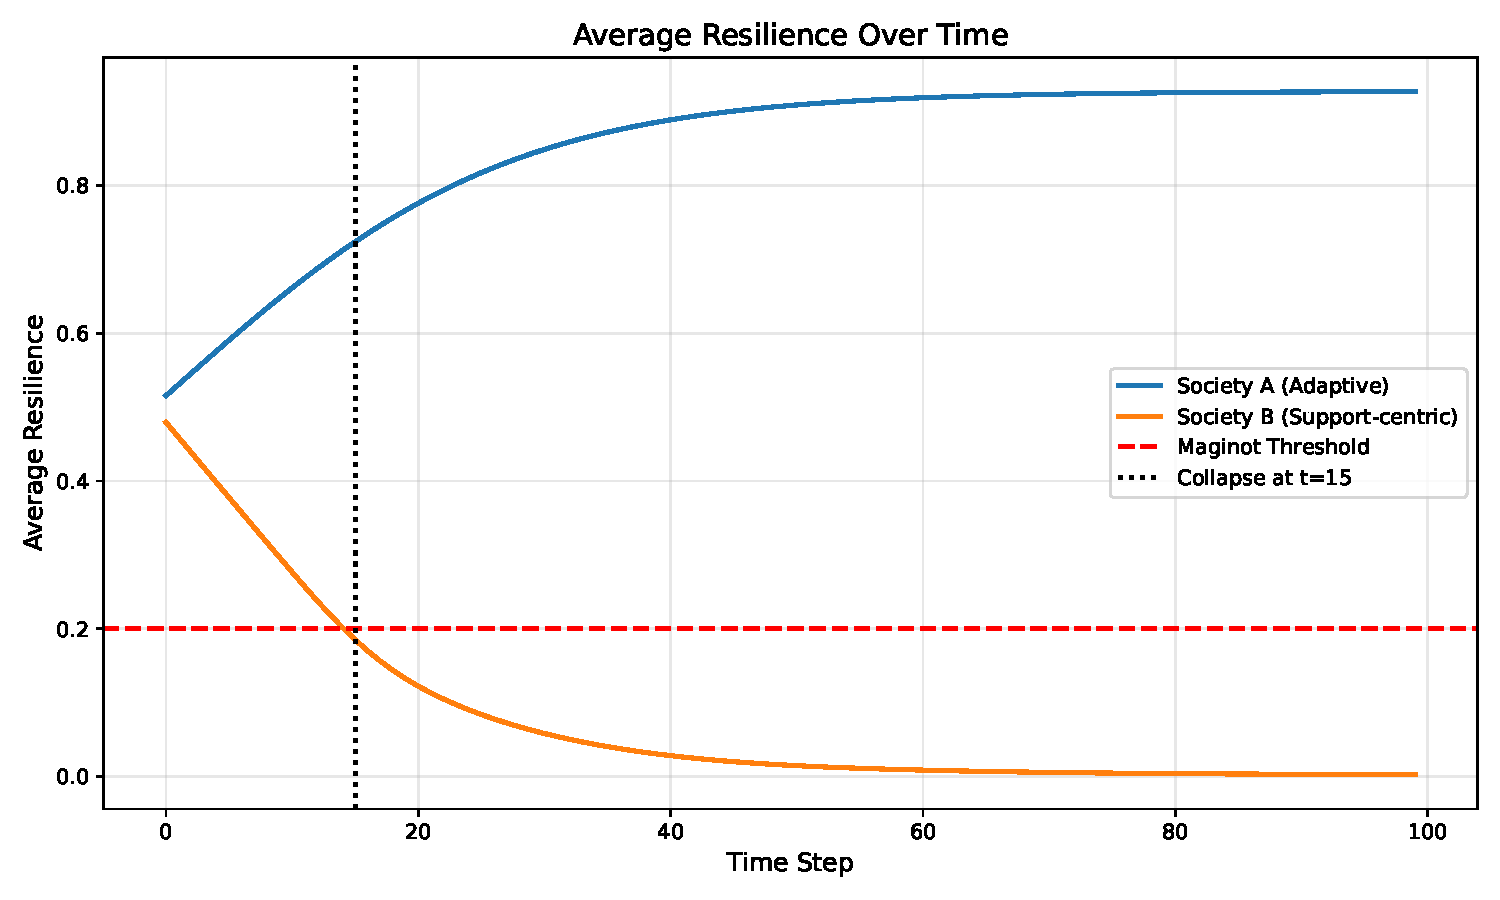
\includegraphics[width=0.8\textwidth]{fig_resilience.pdf}
  \caption{사회 A(적응형/자율 중심)와 사회 B(지원 중심)의 평균 회복탄력성 궤적.
  두 사회 모두 동일한 공감 분포와 초기 회복탄력성에서 시작한다.
  사회 A는 점진적으로 집단화를 줄이고 적절한 스트레스를 회복탄력성 성장으로 전환하여 높은 회복탄력성 균형으로 수렴한다.
  사회 B는 평균 회복탄력성이 감소하며 결국 $t \approx t_{\text{mag}}$에서 임계값 $R_{\text{crit}} = 0.2$를 넘는다.}
  \label{fig:resilience}
\end{figure}

이 예시에서:
\begin{itemize}
  \item 사회 A에서는 $G_t^A$가 $\eta_A$의 비율로 감소하고, $k_A R(1-R)$이 성장을 촉진하며 마모 항은 완만하다.
    시스템은 낮은 집단화와 함께 높은 평균 회복탄력성에서 안정화된다.
  \item 사회 B에서는 높은 스트레스가 $\gamma_B C_t^B$를 통해 $G_t^B$를 증가시키고, 회복탄력성은 $d_B$에 크게 의존하며 $k_B S_i^B$로 인한 누적 마모가 결국 우세해진다.
    평균 회복탄력성은 유한한 시간 $t_{\text{mag}}$에서 문턱값 $R_{\text{crit}}$을 넘는다.
\end{itemize}

이러한 궤적은 섹션~\ref{sec:general}의 더 일반적인 구조적 결과를 구체적으로 예시한다.

\subsection{공감 비선형성 $\alpha$에 대한 민감도}

다음으로 공감 비선형 지수 $\alpha$가 사회 B의 안정성에 어떤 영향을 미치는지 살펴본다.
$\alpha \in [1.0, 1.8]$ 범위의 값들에 대해 사회 B에 대해서만 시뮬레이션을 실행하고 다음을 기록한다:
\begin{itemize}
  \item 최종 평균 회복탄력성 $\bar{R}^B(T)$, 그리고
  \item 붕괴 시간 $t_{\text{mag}}$ (붕괴가 발생하지 않으면 $T$).
\end{itemize}

그림~\ref{fig:sensitivity}는 이 민감도 분석을 시각화한다.

\begin{figure}[t]
  \centering
  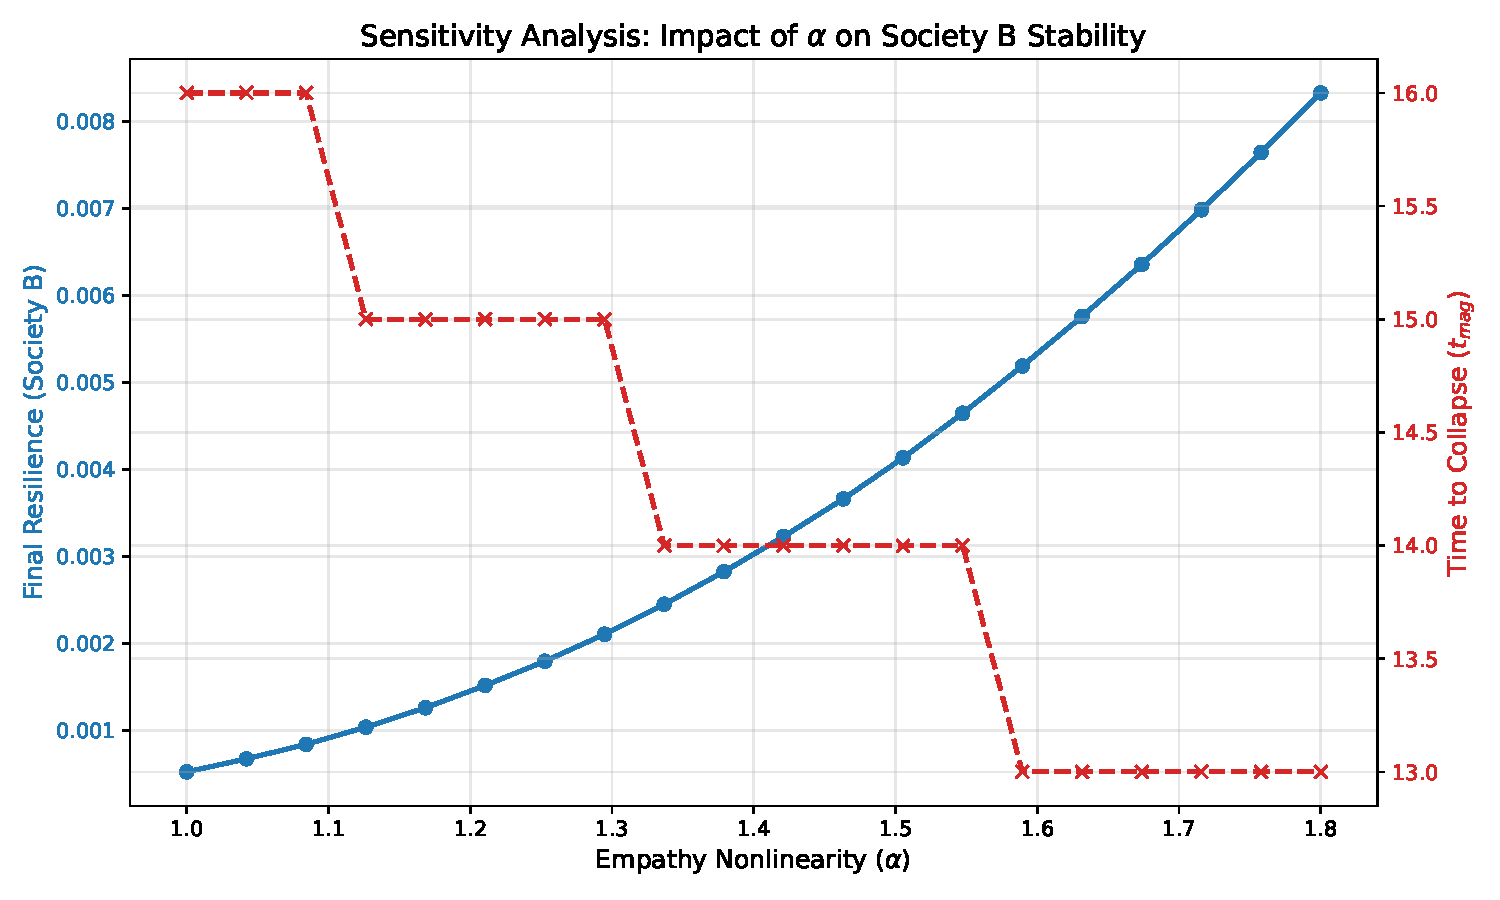
\includegraphics[width=0.8\textwidth]{fig_sensitivity.pdf}
  \caption{공감 비선형 지수 $\alpha$에 따른 사회 B의 민감도.
  청색 실선은 최종 평균 회복탄력성 $\bar{R}^B(T)$을 나타내고, 적색 점선은 붕괴 시간 $t_{\text{mag}}$(붕괴가 없으면 $T$)를 보여준다.
  이 장난감 모델에서 $\alpha$가 클수록 고공감 개인들 사이의 스트레스가 불균형적으로 증가하며, 이는 회복탄력성을 낮추고 붕괴를 앞당기는 경향이 있다.}
  \label{fig:sensitivity}
\end{figure}

이 장난감 설정에서 $\alpha$가 증가하면 고공감 개인들 사이의 스트레스가 선형보다 빠르게 증가하며, 이는 네트워크 이득과 결합되어 지원 중심 체제를 더 취약하게 만든다.

\subsection{네트워크 이득 및 위상에 대한 민감도}
\label{sec:local-coupling}

평균장 모델($G_t$가 전역 스칼라)에 대한 잠재적인 비판은 실제 사회 네트워크의 전형적인 복잡한 클러스터링과 국소적 상호작용을 무시한다는 점이다.
이를 해결하기 위해 우리는 ``좁은 세상(Small-World)'' 네트워크 모델(Watts-Strogatz)을 사용하여 \textbf{국소적 결합(Local Coupling)}을 지원하도록 시뮬레이션을 확장했다.

이 확장된 모드에서는:
\begin{itemize}
    \item 에이전트는 평균 차수 $k=20$ 및 재배선 확률 $p=0.1$을 가진 네트워크의 노드가 된다.
    \item 집단화 $G$는 국소 변수가 된다; 에이전트 $i$의 경우, 전역 평균이 아니라 이웃들의 국소적 불안에 의해 스트레스가 영향을 받는다.
    \item 구체적으로, 사회 B의 스트레스 주도형 집단화 갱신은 인구 평균 대신 $C_{i}^B = \text{mean}(S_{\text{이웃 of } i})$를 사용한다.
\end{itemize}

시뮬레이션 결과, 국소적 클러스터링이 평균장 예측보다 빠르게 스트레스를 증폭시키는 ``공명 구역(pockets of resonance, 반향실)''을 형성함에도 불구하고, 거시적 역학의 본질은 변하지 않았다.
즉, 집단화를 부추기는 정책은 결국 임계점(마지노 시간)을 앞당긴다.

\begin{figure}[h]
  \centering
  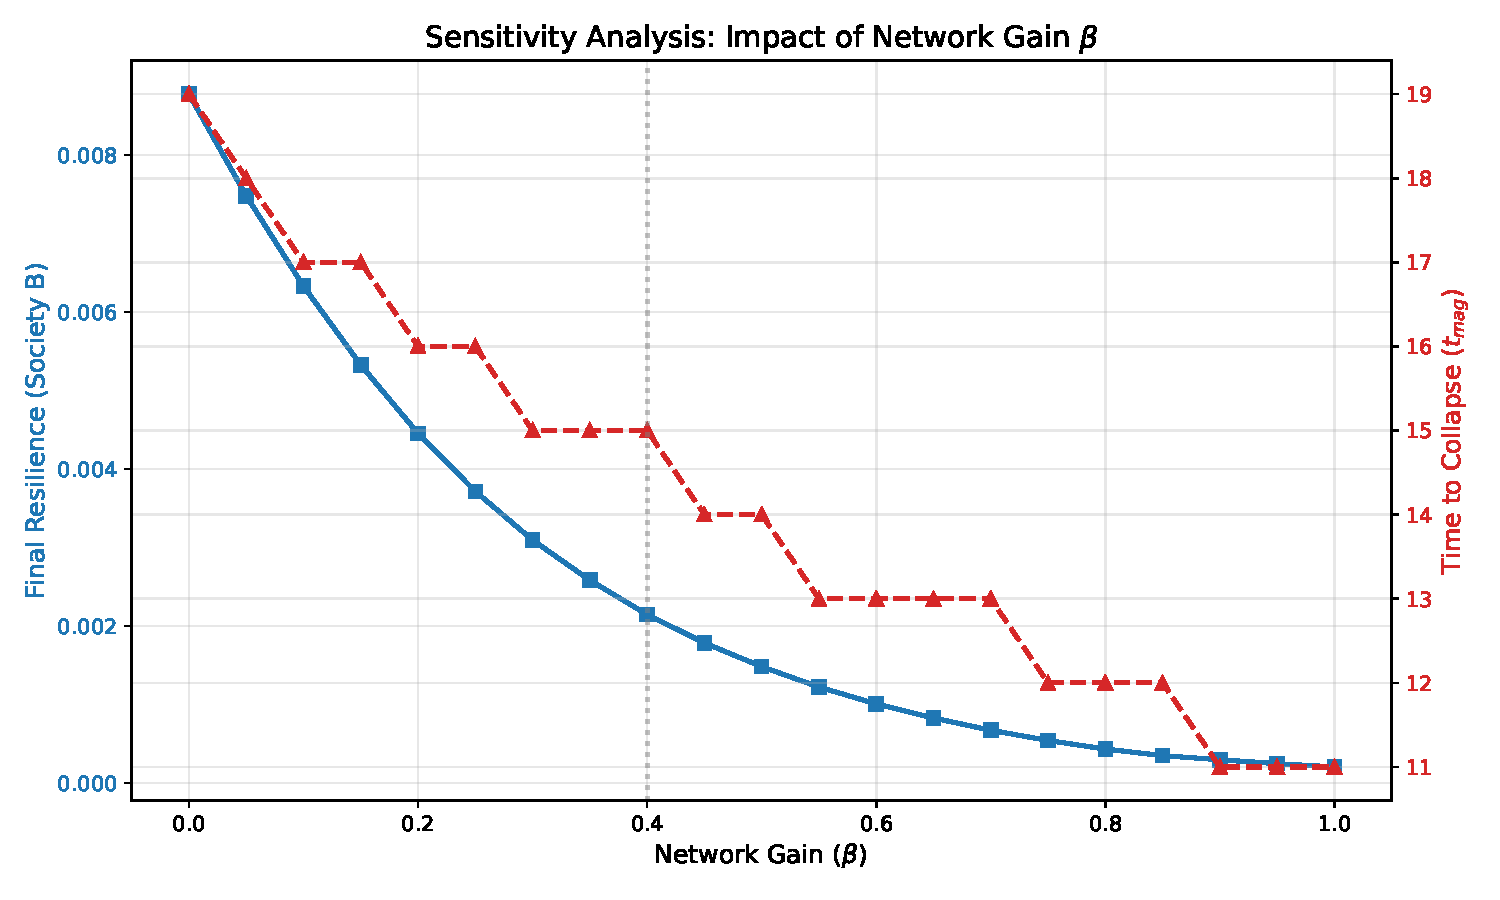
\includegraphics[width=0.8\textwidth]{fig_gain.pdf}
  \caption{지원 중심 체제(사회 B)에서 네트워크 이득($\beta$)이 사회적 안정성에 미치는 영향.
  네트워크 이득 매개변수 $\beta$가 증가함에 따라 시스템의 스트레스 완충 능력은 급격히 감소한다.
  높은 기본 지원($d_B$)이 있더라도, 고이득 환경($\beta > 0.5$)은 마지노 시간의 도래를 가속화한다.
  이 효과는 스트레스가 소실되기 전에 클러스터 내부에서 공명하는 국소적 결합 시나리오에서 더욱 악화된다.}
  \label{fig:gain}
\end{figure}

그림~\ref{fig:gain}은 이득 매개변수 $\beta$의 결정적 역할을 보여준다.
$\beta$가 낮을 때 네트워크는 단순한 매개체에 불과하지만, 임계치를 넘으면 스트레스-집단화의 양의 피드백 루프가 지배하기 시작한다.
이는 ``규모의 역설''이 본질적으로 네트워크의 \emph{이득(gain)}에 기인함을 시사하며, 현대 디지털 기술은 이 이득을 전례 없는 수준으로 끌어올렸다.

\section{마지노 시간과 정책적 해석}
\label{sec:maginot}

주어진 체제와 그룹화 경로에 대해 사회 B의 마지노 시간을 다음과 같이 정의한다:
\[
t_{\text{mag}}^B = \min\{ t \,:\, \bar{R}^B(t) \le R_{\text{crit}}\},
\]
모든 $t < t_{\text{mag}}^B$에 대해 $\bar{R}^B(t) > R_{\text{crit}}$이다.

$t_{\text{mag}}^B$ 이후에는 평균 회복탄력성이 붕괴하여, 미세한 충격에도 시스템이 마비될 수 있다.
이 단계에서는, 대대적인 외부 개입 없이는 단순한 규제( $\beta$ 감소)만으로 회복탄력성을 복구하기 어렵다.

쇠퇴를 지수 함수로 근사하면,
\[
\bar{R}^B(t) \approx R_0 e^{-kt}, \quad k>0,
\]
다음과 같다:
\begin{equation}
t_{\text{mag}}^B \approx \frac{1}{k} \ln\left(\frac{R_0}{R_{\text{crit}}}\right),
\end{equation}
여기서 $k$는 $\alpha, \beta, k_A, \lambda_A, k_B, d_B, \gamma_B$ 그리고 공감 분포의 결합된 효과를 압축한 유효 쇠퇴율이다.
이는 효과적인 개입을 위한 창구가 유한하며 시스템의 내부 피드백 구조에 의해 지배된다는 점을 강조한다.

명제~\ref{prop:maginot}는 구조적 재해석을 더한다: 동일한 체제 매개변수 $\theta$를 공유하지만 그룹화 경로가 다른 모든 정책들 중에서, 체계적으로 그룹화를 낮게 유지하는 정책들은 단조성 가정 하에 약하게 더 큰 $t_{\text{mag}}$을 가질 것이다.
이런 의미에서 그룹 해체를 장려하거나 경직된 정체성 클러스터링을 약화시키는 것은 시스템의 회복탄력성 단계를 확장하기 위한 구조적으로 안전한 방향이다.

\section{토론}

\subsection{콘텐츠와 도덕성을 넘어서}

흔히 공적 담론은 사회적 스트레스의 \emph{콘텐츠}(예: 혐오 표현, 가짜 뉴스)나 공감의 \emph{도덕성}(부족 vs 과잉)에 천착한다.
그러나 이는 문제의 단면일 뿐이다.

본 연구가 시사하는 바는 명확하다. 온건한 콘텐츠라도 고이득 네트워크에서 반복 증폭되면 시스템을 위협할 수 있으며, 그 장기적 파급력은 정책 체제와 집단화 역학에 달려 있다는 것이다:
\begin{itemize}
  \item 이득이 낮고 자율 중심적인 체제(사회 A)에서 공감은 주로 국소적 감쇠 메커니즘으로 작동하며, 적절한 스트레스는 회복탄력성의 적응적 성장을 촉진할 수 있다.
  \item 이득이 높고 지원 중심적인 체제(사회 B)에서 공감은 특히 스트레스가 더 강한 그룹화와 정체성 클러스터링으로 이어질 때 양의 피드백 루프의 일부가 될 수 있다.
\end{itemize}

섹션~\ref{sec:general}의 일반적인 프레임워크와 섹션~\ref{sec:simulation}의 확장된 네트워크 시뮬레이션은 이것이 단지 특정 함수 형태의 산물이 아님을 명확히 한다.
그룹화가 스트레스를 줄이지 않고 스트레스가 회복탄력성을 개선하지 않는 한 구조적으로 다음과 같다:
\begin{itemize}
  \item 더 높은 그룹화는 항상 회복탄력성에 약하게 더 나쁘다.
  \item 매 시점마다 그룹화를 줄이는 어떠한 정책 조합도 도움이 될 뿐이다.
\end{itemize}

따라서 문제의 핵심은 ``공감의 유무''나 ``콘텐츠의 선악''이 아니라, \textbf{공감, 콘텐츠, 네트워크 이득, 그리고 집단화가 상호작용하는 구조적 메커니즘}에 있다.

\subsection{동적 설계 선택으로서의 정책 체제}

사회 A와 사회 B의 대조는 실제 사회를 ``좋다''거나 ``나쁘다''고 낙인찍기 위한 것이 아니다.
오히려 그것은 여러 축에 걸친 두 가지 이상적인 극단을 나타낸다:
\begin{itemize}
  \item 개인적 도전 대 스트레스에 대한 외부적 완충,
  \item 집단 정체성에 대한 약화 대 강조,
  \item 장기적 회복탄력성 구축 대 단기적 구제.
\end{itemize}

이득이 낮고 결합이 약한 환경에서는 두 체제 모두 상당히 안정적일 수 있다.
그러나 높은 이득과 강한 결합 하에서 외부적 완충과 집단 기반 반응에 크게 의존하는 체제는 진화적 수준의 공감 분포가 존재할 때 더 빨리 취약해질 수 있다.

일반화된 구조적 분석 결과는 하나의 설계 원칙을 강력하게 지지한다: 공감의 분포나 자원의 배분과 무관하게, \textbf{집단화를 완화하고 경직된 정체성 형성을 억제하는 것}이 회복탄력성에 유리하다는 점이다.
공감이나 보호 정책 자체가 문제는 아니다. 결정적인 변수는, 그것이 집단화와 네트워크 이득을 증폭시키는 방향으로 작동하느냐이다.

\section{한계 및 향후 연구}

이 프레임워크는 의도적으로 단순화되었으며 몇 가지 중요한 한계가 있다:

\begin{enumerate}
  \item \textbf{모델의 단순성.}  
  함수 형태는 해석의 용이성을 위해 선택되었다.
  실질적인 적용을 위해서는 더 현실적인 비선형성, 이질성, 그리고 상호작용 항이 필요할 것이다.

  \item \textbf{실증적 캘리브레이션의 부재.}  
  매개변수들은 데이터에 맞춘 것이 아니라 개념적 설명을 위해 선택되었다.

  \item \textbf{규범적 주의사항.}  
  이 모델은 공감, 복지, 보호 정책, 또는 정체성 기반 조직화가 본질적으로 해롭다고 주장하지 않는다.
  다만 특정 구조적 조합과 단조성 가정 하에, 그것들이 강한 그룹화 및 높은 이득과 긴밀하게 결합될 때 의도치 않게 불안정성에 기여할 수 있음을 강조할 뿐이다.

  \item \textbf{범위.}  
  이 논문의 기여는 포괄적인 이론이라기보다 개념적인 출발점에 가깝다.
\end{enumerate}

향후 연구는 다음과 같은 방향으로 진행될 수 있다:
\begin{itemize}
  \item 스트레스에 기반하여 연결선이 진화하는(위상과 상태의 공진화) 명시적 동적 네트워크 그래프로 스칼라 $G_t$를 대체,
  \item 집단 간 이질적인 정책 반응 통합,
  \item 그리고 모델의 질적 예측을 서로 다른 제도적 및 문화적 환경의 데이터와 검증.
\end{itemize}

\section{결론}

본 연구는 공감, 네트워크 이득, 집단화, 정책 체제를 하나의 동역학적 틀로 엮어냈다.
조상들의 저이득 환경에서 `국소적 충격 흡수 장치'였던 공감은, 현대의 고이득 네트워크에서 정책 기조(사회 A vs B)에 따라 전혀 다른 결과를 낳는다.

이 장난감 모델 내에서 마지노 시간—특정 구성 하에서 시스템이 회복을 위한 구조적 능력을 상당 부분 상실하게 되는 유한한 지평—이 나타난다.
좀 더 추상적인 수준에서, 우리는 약한 단조성 가정 하에 모든 시점에서 그룹화를 낮게 유지하는 어떠한 정책 궤적도 체제의 세부 사항이나 공감 분포에 관계없이 회복탄력성을 약하게 개선하고 붕괴를 지연시킴을 보여주었다.

우리는 이 논의가 단순한 도덕적 당위를 넘어, 피드백 루프와 이득, 그리고 동역학에 대한 냉철한 구조적 이해 위에서 이루어지기를 기대한다.
본 프레임워크가 향후 사회 정책, 정신 건강, 플랫폼 설계에 관한 논쟁에서 유용한 개념적 도구가 되기를 바란다.

\appendix

\section{Python 시뮬레이션 코드}
\label{app:code}

다음 Python 코드는 섹션~\ref{sec:local-coupling}에서 논의된 두 가지 체제의 역학, 민감도 분석, 그리고 확장된 \textbf{국소적 결합 / 네트워크 모드}를 구현한다.
이 코드는 섹션~\ref{sec:general}에서 설명한 더 일반적인 단조성 프레임워크의 한 구체적인 사례를 인스턴스화한다.

\begin{lstlisting}[language=Python, caption=Social Dynamics Simulation Code]
import numpy as np
import matplotlib.pyplot as plt
from dataclasses import dataclass
from typing import List, Dict, Optional

@dataclass
class SimulationConfig:
    """Configuration parameters for the social dynamics simulation."""
    # Simulation settings
    N: int = 10000
    T: int = 100
    seed: int = 0
    maginot_threshold: float = 0.2

    # Empathy distribution parameters
    mu_A: float = 1.3
    mu_B: float = 1.0
    sigma_E: float = 0.1

    # Stress model parameters
    alpha: float = 1.3
    beta: float = 0.4

    # Initial state
    initial_resilience_mean: float = 0.5
    initial_resilience_std: float = 0.08
    initial_grouping: float = 0.3

    # Society A (Adaptive)
    k_A: float = 0.09
    lambda_A: float = 0.005
    eta_A: float = 0.05

    # Society B (Support-centric)
    k_B: float = 0.03
    d_B: float = 0.02
    eta_B: float = 0.03
    gamma_B: float = 0.005

    # Network / Local Coupling parameters
    use_local_grouping: bool = False
    n_neighbors: int = 20
    rewiring_prob: float = 0.1

def common_plot_style():
    plt.style.use('default')
    plt.rcParams.update({
        'font.family': 'sans-serif',
        'axes.grid': True,
        'grid.alpha': 0.3,
        'lines.linewidth': 2,
    })

class SocialDynamicsSimulation:
    def __init__(self, config: SimulationConfig = SimulationConfig()):
        self.config = config
        self.rng = np.random.default_rng(config.seed)
        self.history: Dict[str, List[float]] = {
            k: [] for k in ['R_A', 'R_B', 'G_A', 'G_B']
        }
        self.t_collapse: Optional[int] = None
        
        self._initialize_population()
        if self.config.use_local_grouping:
             self._initialize_network()
        self._initialize_state()

    def _initialize_network(self):
        """Create a Small-World network adjacency list."""
        N = self.config.N
        k = self.config.n_neighbors
        p = self.config.rewiring_prob
        
        self.neighbors = np.zeros((N, k), dtype=int)
        for i in range(N):
            for j in range(1, k // 2 + 1):
                self.neighbors[i, j-1] = (i + j) % N
                self.neighbors[i, k // 2 + j - 1] = (i - j) % N
        
        mask = self.rng.random(self.neighbors.shape) < p
        random_neighbors = self.rng.integers(0, N, size=self.neighbors.shape)
        self.neighbors = np.where(mask, random_neighbors, self.neighbors)

    def _initialize_population(self):
        N = self.config.N
        is_high_empathy_group = self.rng.random(N) < 0.5
        mu = self.config.mu_B + is_high_empathy_group * \
             (self.config.mu_A - self.config.mu_B)
        self.E = self.rng.normal(mu, self.config.sigma_E, size=N)
        self.E = np.clip(self.E, 0.0, None)

    def _initialize_state(self):
        N = self.config.N
        R_init = self.rng.normal(
            self.config.initial_resilience_mean, 
            self.config.initial_resilience_std, 
            size=N
        )
        R_init = np.clip(R_init, 0.0, 1.0)
        self.R_A = R_init.copy()
        self.R_B = R_init.copy()
        
        if self.config.use_local_grouping:
            self.G_A = np.full(N, self.config.initial_grouping)
            self.G_B = np.full(N, self.config.initial_grouping)
        else:
            self.G_A = self.config.initial_grouping
            self.G_B = self.config.initial_grouping

    def calculate_stress(self, G):
        return (self.E ** self.config.alpha) * (1 + self.config.beta * G)

    def step(self, t: int):
        S_A = self.calculate_stress(self.G_A)
        S_B = self.calculate_stress(self.G_B)

        # Update Resilience
        self.R_A = (self.R_A
                    + self.config.k_A * self.R_A * (1 - self.R_A)
                    - self.config.lambda_A * S_A)
        self.R_B = (self.R_B
                    - self.config.k_B * S_B
                    + self.config.d_B)
        
        self.R_A = np.clip(self.R_A, 0.0, 1.0)
        self.R_B = np.clip(self.R_B, 0.0, 1.0)

        # Social Cost & Update Grouping
        if self.config.use_local_grouping:
            neighbor_stress = S_B[self.neighbors]
            C_B_local = neighbor_stress.mean(axis=1)
            
            self.G_A = np.maximum(0.0, self.G_A * (1 - self.config.eta_A))
            self.G_B = np.maximum(
                0.0, 
                self.G_B + self.config.gamma_B * C_B_local - self.config.eta_B * self.G_B
            )
            self.history['G_A'].append(self.G_A.mean())
            self.history['G_B'].append(self.G_B.mean())
        else:
            C_B = S_B.mean()
            self.G_A = max(0.0, self.G_A * (1 - self.config.eta_A))
            self.G_B = max(
                0.0, 
                self.G_B + self.config.gamma_B * C_B - self.config.eta_B * self.G_B
            )
            self.history['G_A'].append(self.G_A)
            self.history['G_B'].append(self.G_B)
        
        self.history['R_A'].append(self.R_A.mean())
        self.history['R_B'].append(self.R_B.mean())

        if (self.t_collapse is None 
                and self.history['R_B'][-1] < self.config.maginot_threshold):
            self.t_collapse = t

    def run(self):
        for t in range(self.config.T):
            self.step(t)
        return self.history
    
    # Plotting code omitted for brevity but present in repo https://github.com/zotanika/social-dynamics-sim
\end{lstlisting}

\begin{thebibliography}{9}

\bibitem{shannon1948}
C.~E.~Shannon,
``A mathematical theory of communication,''
\emph{Bell System Technical Journal}, vol.~27, pp.~379--423, 623--656, 1948.

\bibitem{lloyd2011evolutionary}
E.~A.~Lloyd,
``Evolutionary mismatch,''
in \emph{Encyclopedia of Evolutionary Biology},
Academic Press, 2011.

\bibitem{forrester1961}
J.~W.~Forrester,
\emph{Industrial Dynamics},
MIT Press, 1961.

\bibitem{forrester1971}
J.~W.~Forrester,
\emph{World Dynamics},
Wright--Allen Press, 1971.

\bibitem{pentland2014}
A.~Pentland,
\emph{Social Physics: How Good Ideas Spread --- The Lessons from a New Science},
Penguin Press, 2014.

\end{thebibliography}

\end{document}
